\documentclass[serif,mathserif]{beamer}
\usepackage{amsmath, amsfonts, epsfig, xspace}
\usepackage{algorithm,algorithmic}
\usepackage{pstricks,pst-node}
\usepackage{multimedia}
\usepackage[normal,tight,center]{subfigure}
\setlength{\subfigcapskip}{-.5em}
\usepackage{beamerthemesplit}
\usetheme{lankton-keynote}

\author[ ]{Using firefox to  make remote communication \quad 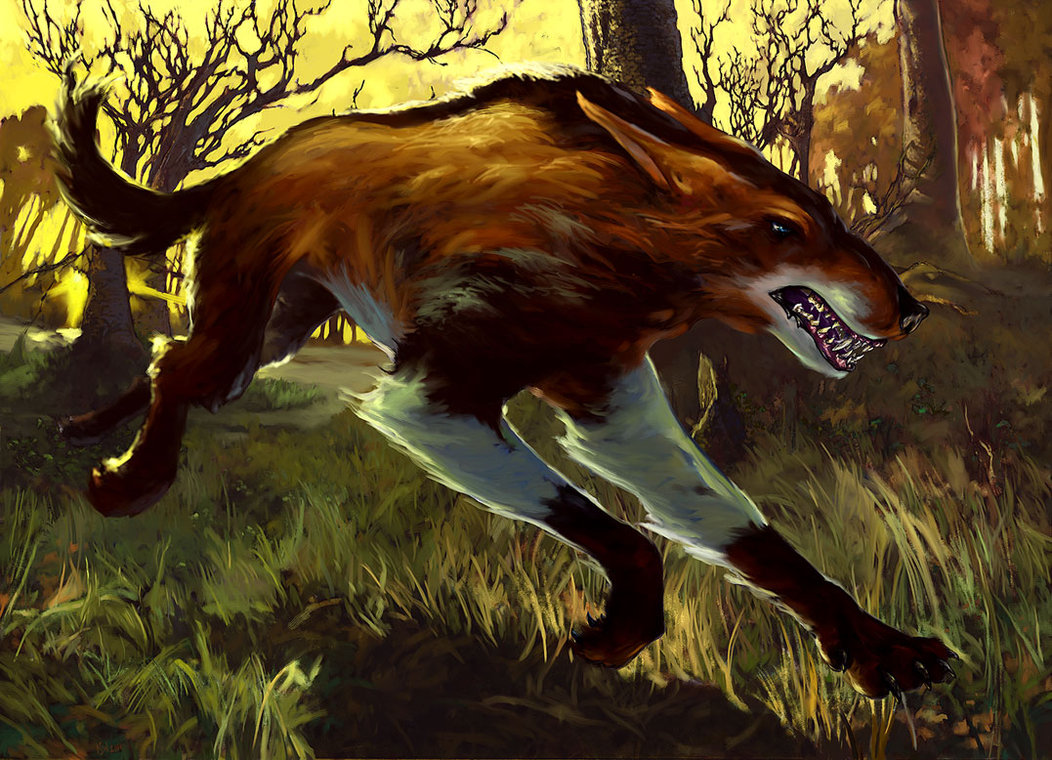
\includegraphics[width=5.0cm]{img/firefoxtunnel.jpg}}

\title[firefox tunnel\hspace{2em}\insertframenumber/\inserttotalframenumber]{Firefox tunnel}

\date{ CoolerVoid - coolerlair@gmail.com - Dezember 21, 2017} %leave out for today's date to be insterted

\institute{Illustration by Anthony S Waters}

\begin{document}

\maketitle
% \section{Introduction}  % add these to see outline in slides
\begin{frame}
  \frametitle{whoami} 
CoolerVoid just another computer programmer and infosec guy.
\end{frame}

\begin{frame}
  \frametitle{Introduction}
  Motivations:\pause
  \begin{itemize}
    \item it's different technique, you can not find in msfvenom, veil...\pause
  \item RedTeam operations.\pause
  \item Improve the work.\pause
  \item Bypass any firewall. %leave out the \pause on the final item
  \end{itemize}
\end{frame}

% \section{Main Body} % add these to see outline in slides

\begin{frame}
  \frametitle{The Justify}
  \begin{itemize}
  \item 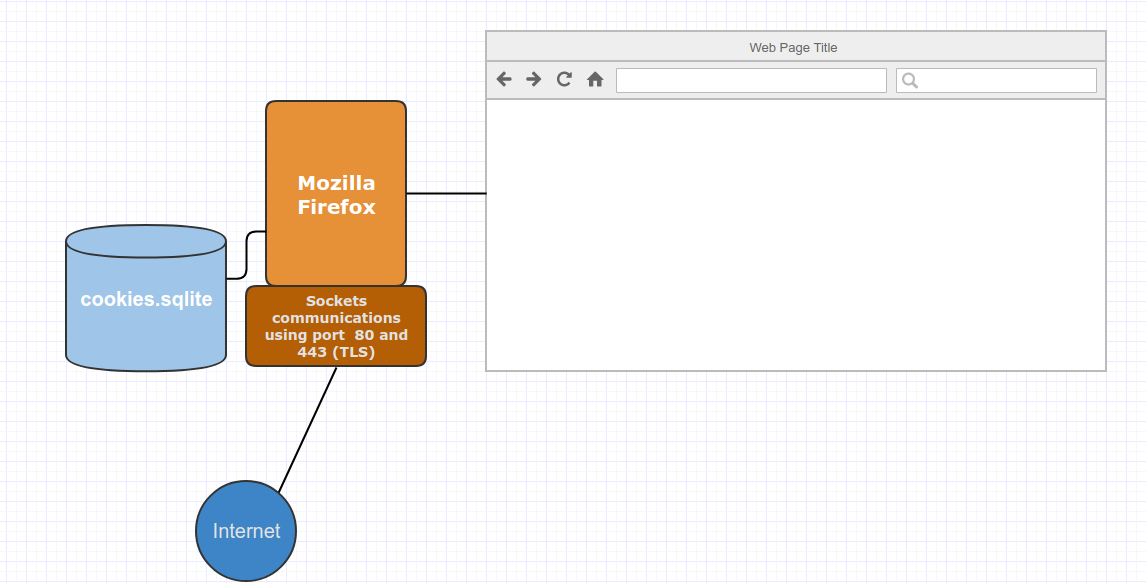
\includegraphics[width=10.0cm]{img/tunnel1.png}
  \end{itemize}
\end{frame}

\begin{frame}
  \frametitle{The Justify}
  \begin{itemize}
  \item 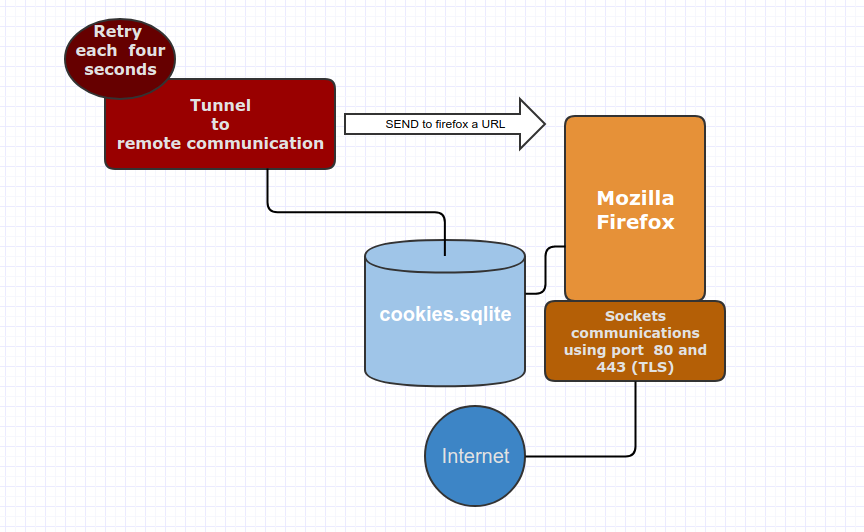
\includegraphics[width=10.0cm]{img/tunnel2.png}
  \end{itemize}
\end{frame}

\begin{frame}
  \frametitle{The Justify}
  \begin{itemize}
  \item 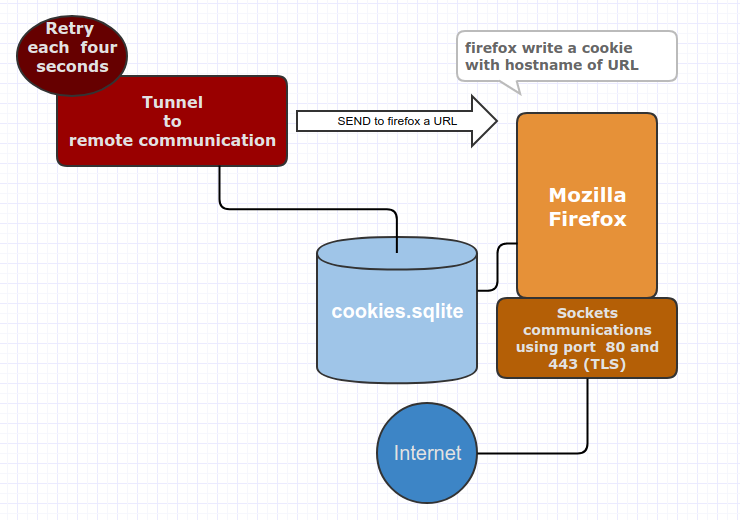
\includegraphics[width=10.0cm]{img/tunnel4.png}
  \end{itemize}
\end{frame}

\begin{frame}
  \frametitle{The Justify}
  \begin{itemize}
  \item 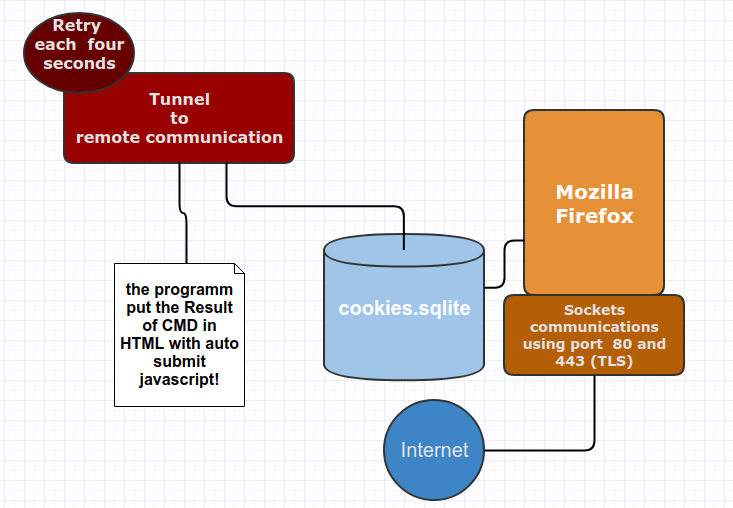
\includegraphics[width=10.0cm]{img/tunnel6.png}
  \end{itemize}
\end{frame}

\begin{frame}
  \frametitle{The Justify}
  \begin{itemize}
  \item 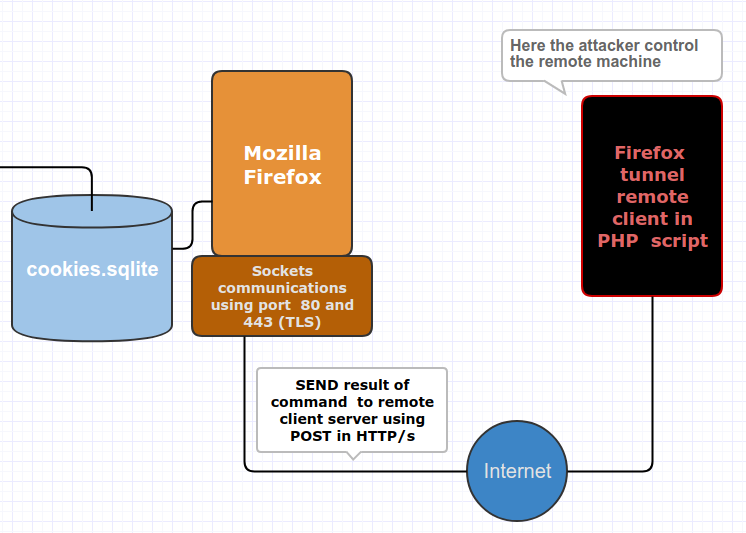
\includegraphics[width=10.0cm]{img/tunnel8.png}
  \end{itemize}
\end{frame}

\begin{frame}
  \frametitle{How too -  Part 1}
  The recipe part 1 the web client:\pause
  \begin{itemize}
  \item Up in your remote host with httpd the directory firefox\char`_shell \pause
  \item Put that directory in root dir of server  example: /var/www/html \pause
  \item Set permissions to write and read in all files of dir... with chmod command...\pause
  \item if you enter in http://machine/firefox\char`_shell/firefox\char`_cmd\char`_tunnel.php?input=1 you can control remote server. %leave out the \pause on the final item
  \end{itemize}
\end{frame}

\begin{frame}
  \frametitle{How too -  Part 2}
  The recipe part 2 - the firefox tunnel server:\pause
  \begin{itemize}
  \item You need mingw32, gcc, c++ and make to build.\pause
  \item At file firefox\char`_tunnel.cpp change line 20 in var domain, replace it to your remote machine IP or DNS. \pause
  \item Set permissions to write and read in all files of dir... with chmod command...\pause
  \item compile in root dir of server with command "mingw32-make", take exe file in directory bin \pause
  \item Execute the file, control him  using the PHP client. \pause
  \item if you enter in http://machine/firefox\char`_shell/firefox\char`_cmd\char`_tunnel.php?input=1 you can control remote  server.  
  \end{itemize}
\end{frame}

% \section{Conclusion} % add these to see outline in slides
\begin{frame}
  \frametitle{Demo}
  \begin{itemize}
  \item At YouTube
  \item Look that following:
  \item https://www.youtube.com/watch?v=C23N4yDRkjU
  \end{itemize}
\end{frame}

\begin{frame}
  \frametitle{Credits}
  \begin{itemize}
  \item Thank you
  \item Any doubt ? talk to me coolerlair@gmail.com
  \item Twitter: @Cooler\char`_freenode
  \item Github: https://github.com/CoolerVoid/
        %http://newsgroups.derkeiler.com/Archive/Comp/comp.text.tex/2007-11/msg00299.html
  \end{itemize}
\end{frame}

\end{document}
